%
%
%
% - - - - - Prototyp - - - - - - - - 
%
%
%
\chapter{Prototyp zur Unterstützung in der Sterilgutversorgung}
\label{ch:Prototyp}
In dieser Arbeit wurde ein Prototyp für die \emph{Realwear hmt-1} implementiert. Die Funktionalität, verwendete Technologien sowie die Implementation werden im Folgenden vorgestellt.
%
%
%
% - - - - - Funktionalität des Prototypen - - - - - - - -
%
%
%
\section{Funktionalität des Prototypen}
Mithilfe des Prototypen sind zwei grundsätzliche Funktionalitäten möglich. Es ist einerseits möglich, aus einer bestehenden Liste von Bildergalerien eine Galerie auszuwählen und anzuzeigen. Andererseits kann eine Slideshow in Form einer JSON-Datei per QR-Code von einem Server geladen werden. Innerhalb der Bildergalerie ist es dann möglich, vor und zurück zu navigieren. 
Slideshowauswahl und Slides sind in einer Listenansicht dargestellt, die es ermöglicht, stets 4-5 Elemente auf einmal anzuzeigen und bei Bedarf weitere Elemente nachzuladen. Dies wird mit einem Vor- und einem Zurückbutton realisiert.

Die andere Hauptfunktionalität betrifft Videos. Es ist möglich,  Videos aufzuzeichnen und dieses abzuspielen. Es ist ebenso möglich, einen QR-Code mit einer Adresse auf ein MP4-Video aufzurufen und dieses Video zu streamen. Innerhalb eines abgespielten Videos ist es möglich, 10 Sekunden vor oder zurück zu spulen und zu pausieren. Zudem ist es möglich, Kapitelmarken zu setzen und in einer eigenen Ansicht zu bearbeiten.

All diese Funktionalitäten können via Sprachsteuerung ausgewählt werden. Dazu müssen die Beschriftungen der Buttons laut vorgelesen werden. Die Brille interpretiert dann diese Eingaben als \emph{Click}-Events und ruft entsprechende Funktionen auf.

In der Praxis können Bilder-Slideshow und Videos eingesetzt werden, um Angestellten der AEMP wichtige Informationen zu medizinischen Instrumenten zu geben. So können Hyperlinks zu Anleitungen per QR-Code oder Barcode auf die Smartglass geladen werden und von einem externen Server gestreamt werden.

Um auch ohne Internetverbindung arbeiten zu können, ist es zu Beginn des Appstarts möglich, eine lokale Server-URL per QR-Code einzulesen. Diese wird anschließend vor alle per QR-Code eingelesenen URLs gesetzt, sodass es möglich ist auch in einer Umgebung wie der AEMP, in der keine Internetverbindung zur Verfügung steht, auf Videos und Bilder eines lokalen Servers zuzugreifen. 

Zum Testen wurde ein lokaler NodeJS-Server aufgesetzt, welcher Mediendaten ausliefert.
%
%
%
% - - - - - Verwendete Technologien - - - - - - - - 
%
%
%
\section{Verwendete Technologien}
\label{sec:Verwendete_Technologien}
% 3 Seiten
Für die Implementierung des Prototypen wurde \emph{Android Studio} mit Android in Version 23 verwendet, da dies die neueste Version ist, die von der \emph{hmt-1} unterstützt wird. Die API der \emph{hmt-1} ermöglicht den Zugriff auf die Hardwarefunktionalitäten sowie auf die Sprachsteuerung der Smartglass. Mittels eines Eintrags \emph{\enquote{android:contentDescription}} können Sprachbefehle zu beliebigen Elementen hinzugefügt werden. Die Elemente reagieren dann auf den im Eintrag angegebenen Sprachbefehl und lösen ein \emph{Click}-Ereignis aus.

Die API der Smartglass hat zudem eine Funktionalität, um Barcodes und QR-Codes auszulesen und den Inhalt zurückzugeben und eine API, um Videos in hoher Auflösung aufzuzeichnen. 

Der Prototyp speichert aufgezeichnete Videos auf dem Gerät und serialisiert das dazugehörige Datenobjekt (vgl. Kapitel \ref{sec:Datenmodell}) auf dem Gerätespeicher. Externe Videos und Bilder werden per JSON-Objekt, welches über einen Link von einem Server geladen wird, geladen. Diese JSON-Objekte enthalten alle notwendigen Informationen. So enthält das JSON-Objekt der Slideshow ein Array aus Objekten mit Namen und URL. Beim Video wird der Name, die URL und die Kapitel mit Namen und Position in Millisekunden gespeichert (vgl. Listing \ref{lst:json_video} und \ref{lst:json_slides}).

Der verwendete lokale Server ist ein NodeJs-Server, welcher über die IP-Adresse und den verwendeten Port einen Ordner auf dem Dateisystem freigibt.
%
%
%
% - - - - - Implementation - - - - - - - - 
%
%
%
\section{Implementierung}
\label{sec:Implementation}
Im Folgenden wird die Implementierung des Prototypen beschrieben. 

Das Programm folgt bei der Videofunktionalität dem Model-View-Controller (\emph{MVC})- Pattern, bei dem eine Trennung von Programmlogik, Model und View eingehalten wird.
%
%
%
% - - - - - User-Interface - - - - - - - - 
%
%
%
\subsection{User-Interface (View)}
Die Android-Anwendung wurde nach dem in Abbildung \ref{fig:Storyboard_des_Prototypen} gezeigten Storyboard erstellt. Die Anwendung beginnt in einem Hauptmenü, welches ermöglicht, per Sprachbefehl einen von zwei Buttons auszuwählen. Mit dem ersten Button wird der Nutzer zur Slideshow-Seite weitergeleitet. Beim zweiten Button wird auf die Videoanzeige und beim dritten Button auf die Video-Aufzeichnen Funktion weitergeleitet. Mittels eines \enquote{Schritt-Zurück-Befehls} der Smartglass wird der androidtypische \enquote{Zurückbefehl} betätigt.

\begin{figure}[htbp]
    \centering
    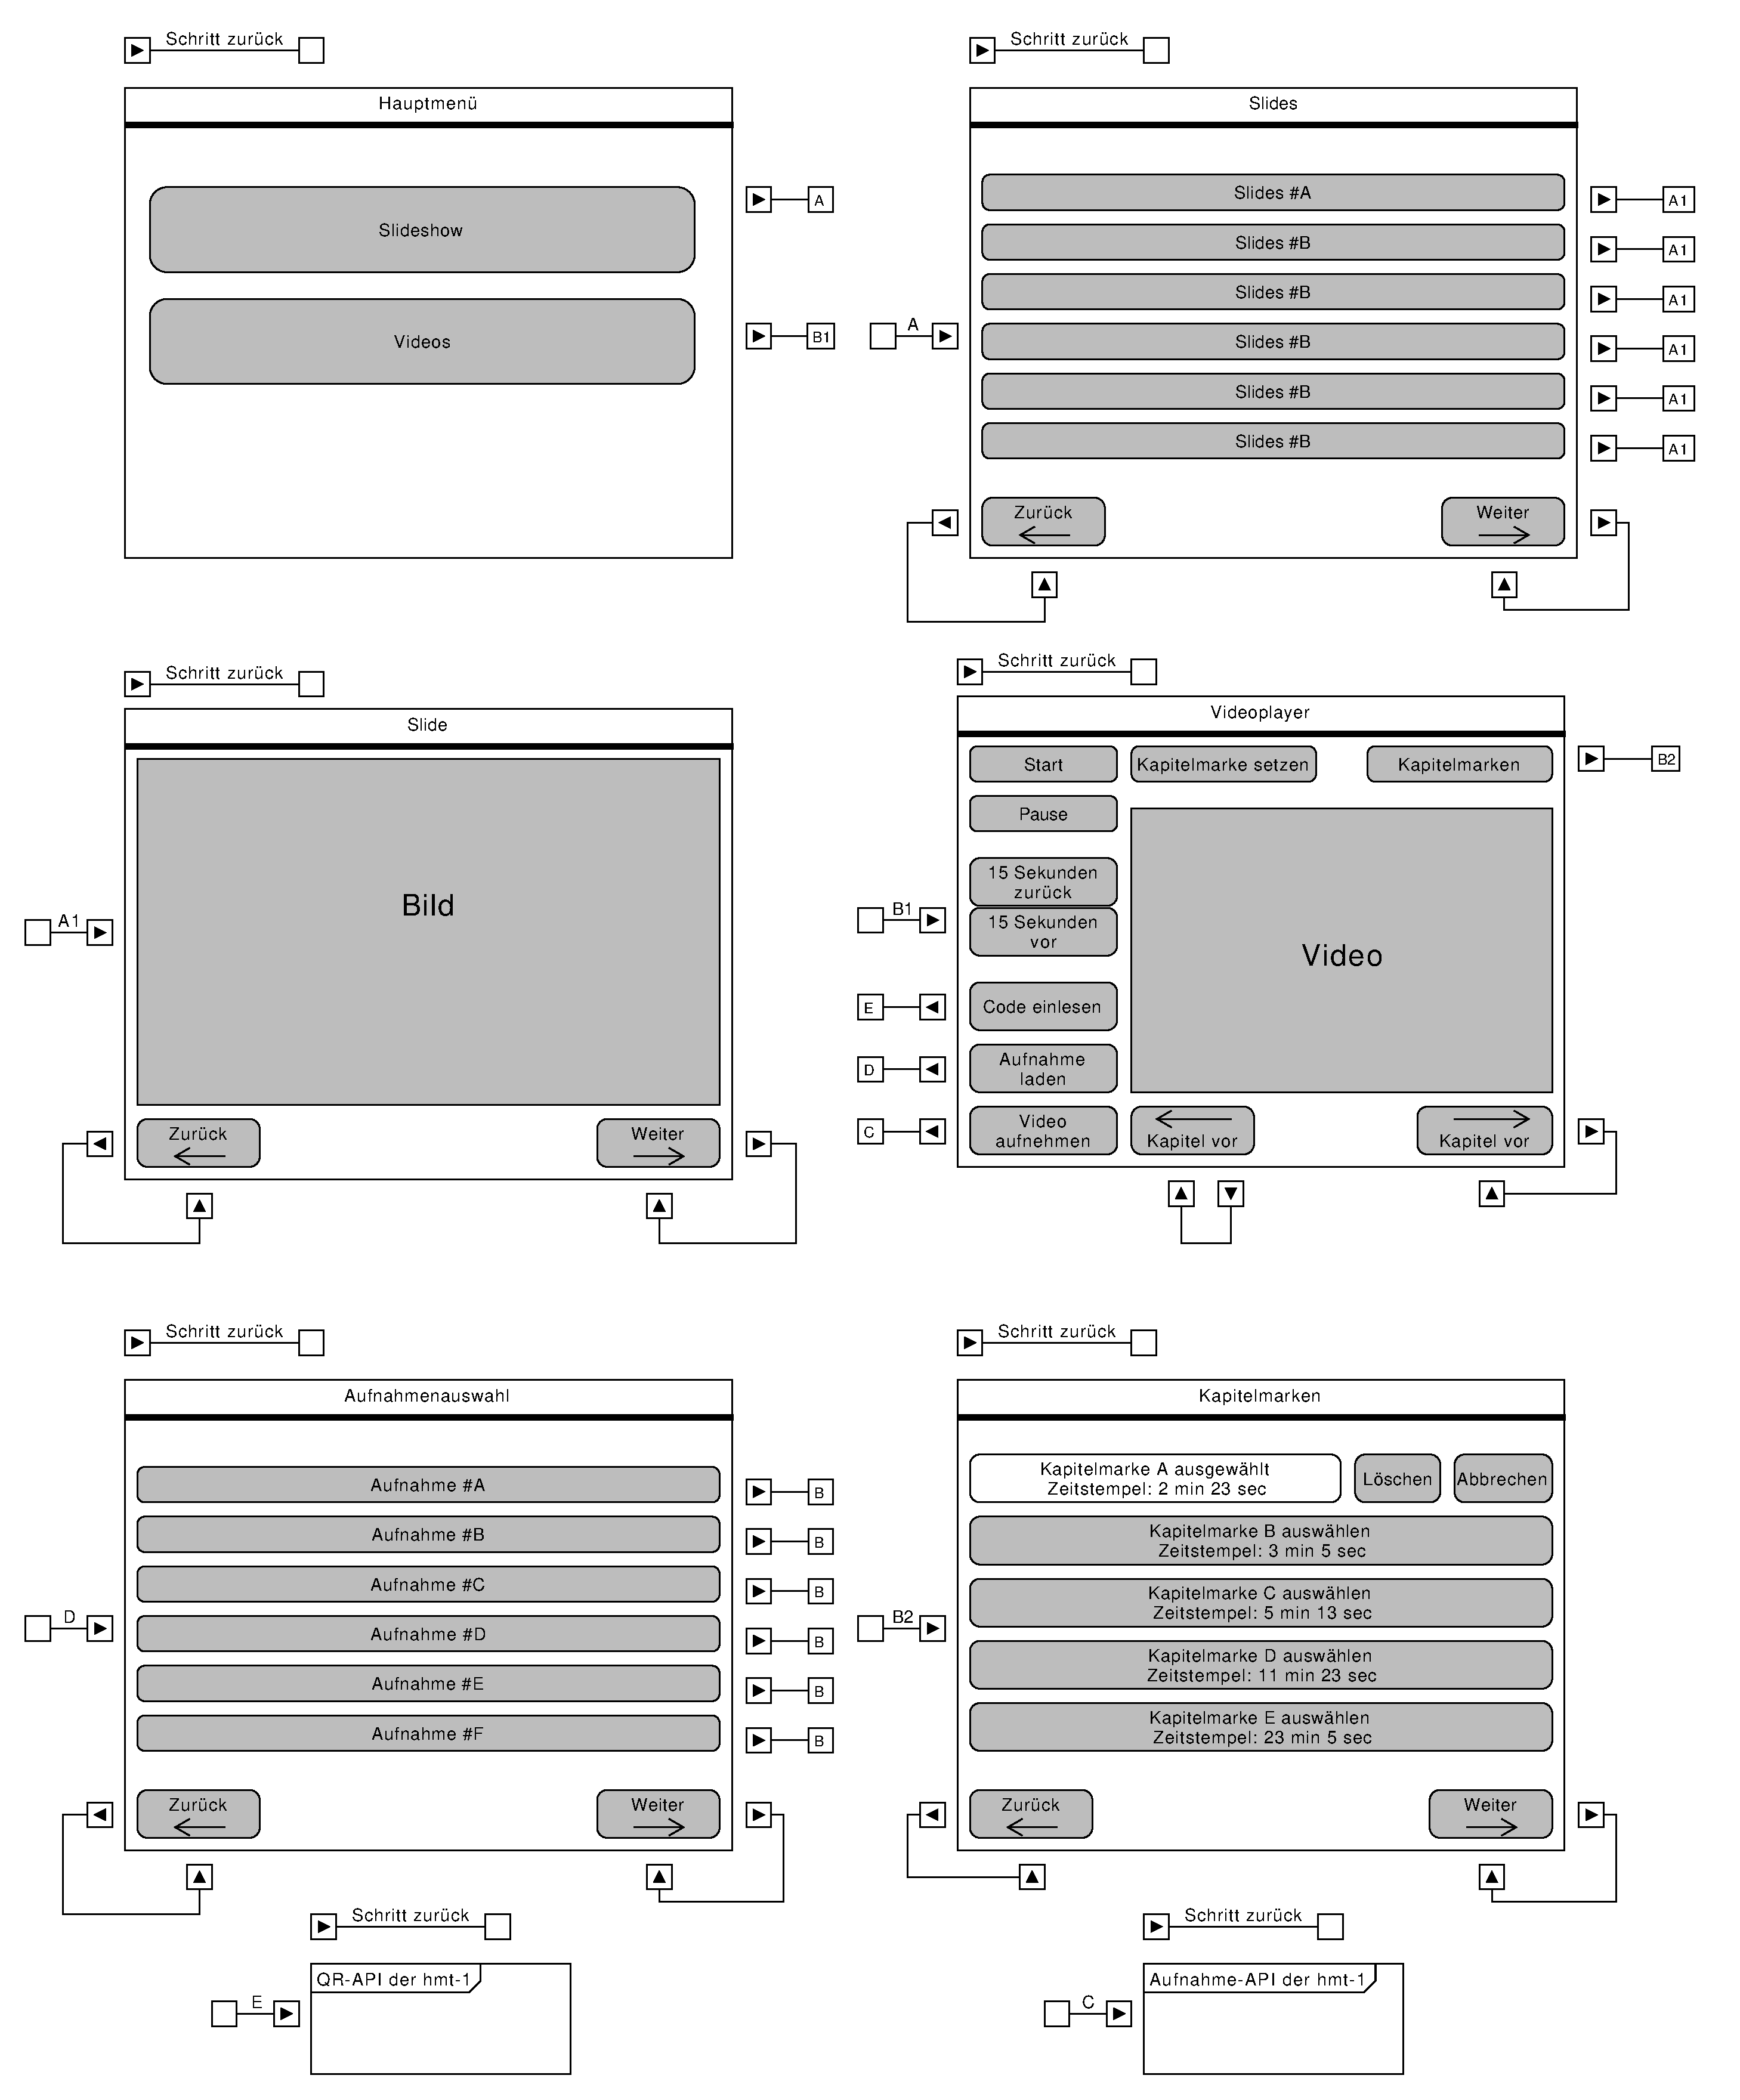
\includegraphics[width=1\textwidth]{data/bilder/UI-Storyboard.pdf}
    \caption{Storyboard des Prototypen}
    \label{fig:Storyboard_des_Prototypen}
\end{figure}

Die Slideshow besteht aus zwei Ansichtstypen. In der ersten Ansicht, welche über das Hauptmenü erreichbar ist, wird eine Liste von Buttons angezeigt, über die einzelne Slides ausgewählt werden können. Am unteren Rand des Fensters ist ein \enquote{Weiterbutton}, welcher die Liste der Buttons aktualisiert, um weitere Slides zur Auswahl zu stellen. Dies ist notwendig, da bei der \emph{hmt-1} klassisches scrollen durch eine Liste nicht möglich ist. Es ist lediglich das Scrollen durch eine kurze Liste per Kopfgesten möglich.

Über einen Button \enquote{Code einlesen} ist es möglich, einen QR-Code zu lesen, der einen Link zu einer JSON-codierten Slideliste kapselt und es so ermöglicht, die Slides dynamisch nachzuladen.

Wird eine Bilderliste ausgewählt, so wird auf eine Unterview verlinkt. Diese besteht aus einer \emph{Image-View} sowie zwei Buttons: \enquote{vorwärts} und \enquote{zurück}. Im Bild wird das aktuelle Bild der Bilderliste angezeigt. Mit \enquote{weiter} wird das nächste, mit \enquote{zurück} das vorherige Bild angezeigt.

Aus der Haupt-Einstiegsview kann zudem die \emph{Videoplayer}-View geöffnet werden. Diese Ansicht besteht aus zwei Bereichen. Links ist eine Sammlung von insgesamt 7 Buttons zum starten und stoppen, vor- bzw. zurückspulen des Videos um 10 Sekunden, Einlesen eines QR-Codes und Einlesen des Videolinks in den Videoplayer. Diese Buttons werden dynamisch ein- bzw ausgeblendet, je nach Stadium, in dem die App sich befindet. So werden immer nur die Buttons angezeigt, die wirklich verwendet werden können. Zusätzlich sind noch zwei Buttons zum Aufnehmen eines Videos und zum Laden einer Aufnahme in den Player. Rechts ist ein Videofenster angebracht, in dem die Videos angezeigt werden.

Einlesen des QR-Codes sowie die Aufnahme des Videos werden mithilfe der API der \emph{hmt-1} realisiert. Der eingelesene Link enthält ein JSON-Objekt, welches den Link sowie die Kapitel enthält. Das Ergebnis wird in der View angezeigt.

Ist ein Video geladen, so werden die Buttons zur Bearbeitung und Verwendung der Kapitelmarken sichtbar. Mittels zweier Buttons an der unteren Bildschirmseite ist es möglich, die jeweils nächsten und vorherigen Kapitelmarken anzusteuern. Mit einem Button an der oberen Bildschirmhälfte ist es möglich, eigene Kapitelmarken an der aktuellen Position des Videos zu setzen. Diese können mittels Spracheingabe benannt werden.

Wird ein Button \enquote{Kapitel} aufgerufen, so wird eine eigene View zur Verwaltung von Kapitelmarken angezeigt, die ähnlich der Slideshowauswahl funktoniert. Hier wird eine Liste angezeigt, in der alle Kapitel aufgelistet werden. Wählt der Nutzer ein Kapitel aus, so erscheinen \enquote{Löschen}- und \enquote{Abbrechen}-Buttons. Mittels \enquote{Löschen} kann das ausgewählte Kapitel gelöscht werden. 
%
%
%
% - - - - - Datenmodell - - - - - - - - 
%
%
%
\subsection{Datenmodell (Model)}
\label{sec:Datenmodell}
In Abbildung \ref{fig:Klassendiagramm} ist neben der Klassenstruktur des Controllers das Klassendiagramm des Models gezeigt. Dieses besteht aus insgesamt vier Klassen: den Basisdatentypen \enquote{Slide}, \enquote{Video} sowie \enquote{VideoChapter} und der Liste von Slides \enquote{SlideList}. 

Die Klasse \enquote{Slide} kapselt einen String \enquote{fileURL} und den Titel \enquote{title}. 
Die Klasse \enquote{VideoChapter} dient zur Speicherung eines Kapitels eines Videos und wird von der Klasse Video verwendet. Ein VideoChapter besteht aus einer Ganzzahl \enquote{position} und dem Namen des Kapitels als String. Die Klasse \enquote{SlideList} kapselt eine \emph{ArrayList} von Slides sowie den Namen der SlideList.
Die Klasse \enquote{Video} besteht aus dem Namen der Datei, in welcher das Video im Dateisystem gespeichert wird, der URL des Videos, dem Titel, sowie aus einer ArrayList von VideoChapter. Video besitzt zudem öffentliche Methoden zum Hinzufügen und Entfernen von Kapiteln sowie zum Persistieren und laden des Video-Models im Dateisystem.
\begin{figure}[htbp]
    \centering
    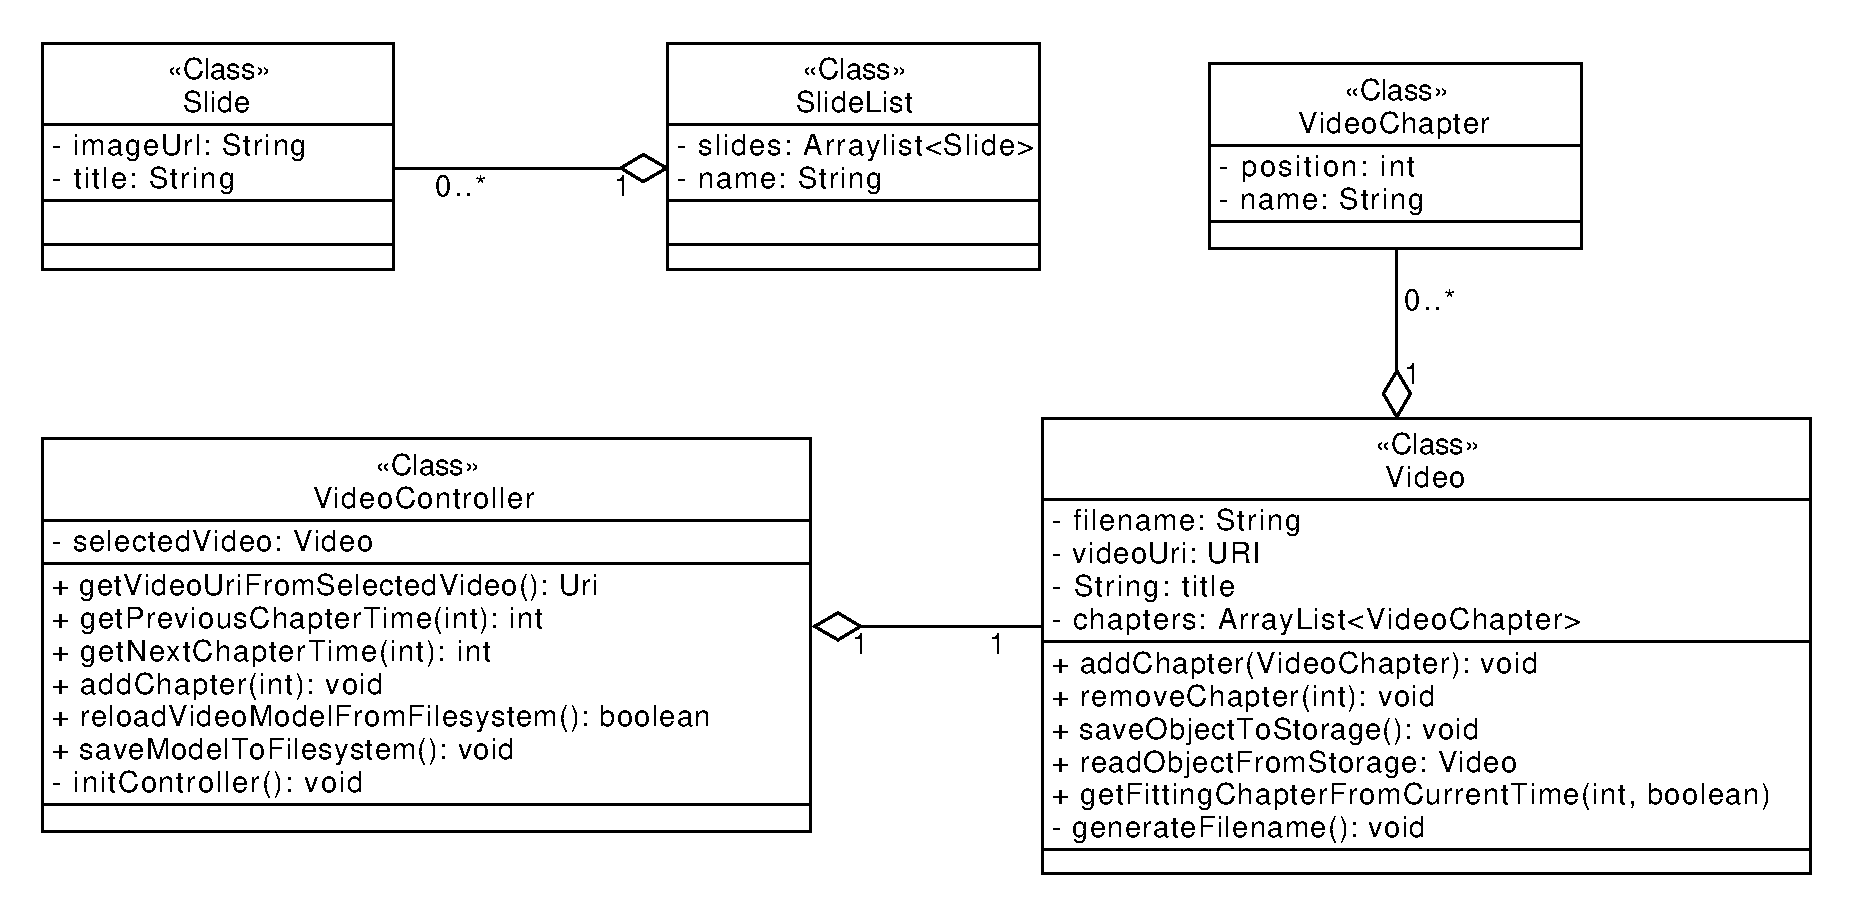
\includegraphics[width=1\textwidth]{data/bilder/Klassendiagramm.pdf}
    \caption{Klassendiagramm der Modelklassen sowie der Controllerklasse}
    \label{fig:Klassendiagramm}
\end{figure}

Die Slides sowie das Video können per Link auf ein JSON-Codiertes Model eingelesen werden. Die Struktur der JSON-Objekte ist in Listing \ref{lst:json_video} und \ref{lst:json_slides} dargestellt.
%
%
%
% - - - - - Programmlogik - - - - - - - - 
%
%
%
\subsection{Programmlogik (Controller)}
Die Programmlogik der Videofunktionalität wird durch einen Controller (vgl. Abbildung \ref{fig:Klassendiagramm}) durchgeführt. Dieser kapselt das Model, also ein Objekt der Klasse Video namens \enquote{selectedVideo}. Mittels verschiedener öffentlicher Methoden kann die Programmlogik realisiert werden. 

\texttt{getVideoURIFromSelectedVideo()} liefert zum gekapselten Model eine Java-URI, die anschließend in der View eingebunden werden kann.

\texttt{getPreviousChapterTime(int)} und \texttt{getNextChapterTime(int)} liefern das nächste Kapitel sowie das vorherige Kapitel abhängig von einer aktuellen Zeit. 

\texttt{addChapter(int)} fügt ein Kapitel zur übergebenen Zeit zum gekapselten Video hinzu. 
\texttt{reloadVideoModelFromFilesystem()} und \texttt{saveModelToFilesystem()} laden bzw. speichern das Model in serialisierter Form im Dateisystem.

Die Slideshow wird per HTTP-Request geladen und aus einem JSON-Objekt (vgl. Listing \ref{lst:json_slides}) in ein Java-Objekt umgewandelt. Es ist ebenso möglich, eine Slideshow aus einem auf einem externen Server liegenden JSON-Datei per QR-Code zu laden. Die Bilder der Slideshow werden von einem Server geladen.

Videos können ebenfalls per HTTP-Request geladen werden und aus einem JSON-Objekt (vgl. Listing \ref{lst:json_video}) in ein Java-Objekt umgewandelt. 

\begin{minipage}{\linewidth}
\begin{lstinputlisting}[%
    caption={JSON-Struktur des Videos},%
    captionpos=b, %
    label={lst:json_video},%
    language=json,%
    firstnumber=1, %
    basicstyle=\scriptsize, %
    breaklines=true]
{sourcecode/jsonStruktur_video.json}
\end{lstinputlisting}
\end{minipage}
%
\begin{minipage}{\linewidth}
\begin{lstinputlisting}[%
    caption={JSON-Struktur der Slides},%
    captionpos=b, %
    label={lst:json_slides},% 
    language=json,%
    firstnumber=1, %
    basicstyle=\scriptsize, %
    breaklines=true]
{sourcecode/jsonStruktur_slides.json}
\end{lstinputlisting}
\end{minipage}
%
%
%
% - - - - - Lokaler Server - - - - - - - - 
%
%
%
\subsection{Lokaler Server}
\label{sec:Lokaler_Server}
Als lokaler Server wird ein NodeJs-Server verwendet. Dieser liefert Zugriff auf alle in einem Ordner \enquote{Public} liegenden Dateien. So lassen sich URLs erstellen und per QR-Code von der Smartglass aus laden, die direkte Links zu Dateien enthalten.

Die Bilder werden zur Anzeige heruntergeladen, die Videos werden gestreamt. Zum Streamen wird die URL des Videos in eine \emph{URI} überführt und dem Android-Videoplayer übergeben. Mithilfe des Videoplayer-Steuerelementes der Android-Api werden die Videoinhalte gestreamt.

Aufgerufen wird der Server über zwei QR-Codes. Der erste Code initialisiert den Server auf dem Client. Die Server-Basis-URL wird zunächst beim Appstart durch einen QR-Code geladen. Dieser enthält die IP-Adresse des Servers sowie den Port, über den die Serveranwendung angesprochen wird. In den QR-Codes von Slidelists sowie Videos werden lediglich die Unterpfade gekapselt, welche zur entsprechenden Datei führen. Innerhalb der Smartglass-Anwendung werden Pfad zum Server und zum Unterpfad zusammengesetzt.

Die Hauptadresse des Servers wird mithilfe einer statischen Hilfsklasse innerhalb des Smartglass-Prototypen gespeichert und ist somit in allen Ansichten der App verfügbar.